%% Be aware of the * 

\chapter*{Introduction}

A document store or document-oriented database system, is a storage concept characterized by its schema-free organization of data \autocite{solidit2019}. 
A document store can contain several collections, each of which contains one or more records/documents as shown in figure \ref{fig:docstore1} \autocite{mongodb2019}.

\begin{figure}[ht]
    \centering
    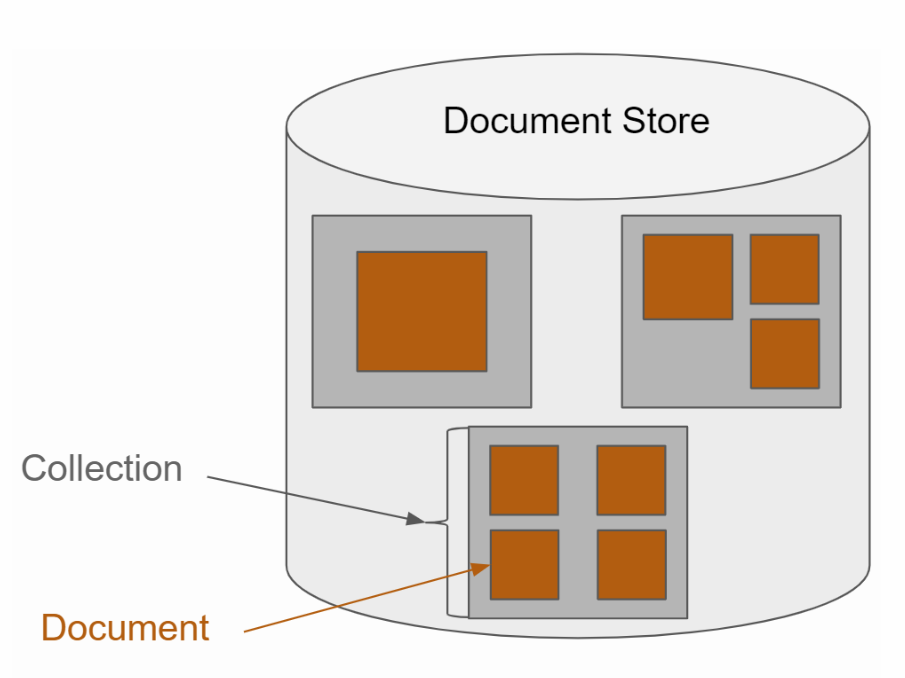
\includegraphics[width=0.5\textwidth]{DocumentStore1.png}
    \caption{Document store architecture}
    \label{fig:docstore1}
\end{figure}

According to \autocite{solidit2019}, unlike relational database systems, document stores allow a non-uniform structure of their records. This means that each record can have individual columns. Furthermore the data types of the different columns can be different from record to record. 

Contrary to relational databases, columns can have multiple values and data records can have a nested structure as shown in figure \ref{fig:docstore2}.

\begin{figure}[ht]
    \centering
    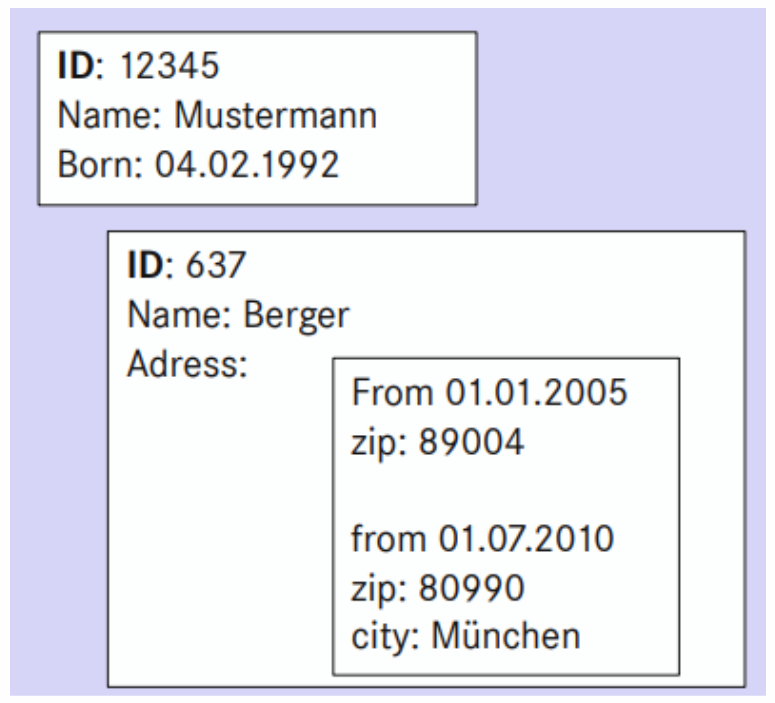
\includegraphics[width=0.5\textwidth]{DocumentStore2.png}
    \caption{Example of two document store records \autocite{buckenhofera.2019}}
    \label{fig:docstore2}
\end{figure}

According to \autocite{solidit2019}, most document stores use notations, which can be easily processed by applications accessing the stored data. The most common data notation is JavaScript Object Notation (JSON) as it supports a key-value serialization of the data without predefining the type of the value \autocite{elastic2019}.
Important examples of document stores are MongoDB, Amazon DynamoDB, Couchbase and CouchDB \autocite{solidit2019}. Elasticsearch primarily is a search engine, which uses a distributed document store as its secondary database model \autocite{solidit2019_02}.
